%%%%%%%%%%%%%%%%%%%%%%%%%%%%%%%%%%%%%%%%%%%%%%%%%%%%%%%%%%%%%%%%%%%%%%%%%%%%%%%%%%%%%%%
%%%%%%%%%%%%%%%%%%%%%%%%%%%%%%%%%%%%%%%%%%%%%%%%%%%%%%%%%%%%%%%%%%%%%%%%%%%%%%%%%%%%%%%
% 
% This top part of the document is called the 'preamble'.  Modify it with caution!
%
% The real document starts below where it says 'The main document starts here'.

\documentclass[12pt]{article}

\usepackage{amssymb,amsmath,amsthm}
\usepackage[top=1in, bottom=1in, left=1.25in, right=1.25in]{geometry}
\usepackage{fancyhdr}
\usepackage{graphicx}
\usepackage{enumerate}
\usepackage{verbatim}
\usepackage{listings}
\usepackage{xcolor}

% Comment the following line to use TeX's default font of Computer Modern.
\usepackage{times,txfonts}

\definecolor{codegreen}{rgb}{0,0.6,0}
\definecolor{codegray}{rgb}{0.5,0.5,0.5}
\definecolor{codepurple}{rgb}{0.58,0,0.82}
\definecolor{backcolour}{rgb}{0.95,0.95,0.92}

\lstdefinestyle{mystyle}{
    backgroundcolor=\color{backcolour},   
    commentstyle=\color{codegreen},
    keywordstyle=\color{magenta},
    numberstyle=\tiny\color{codegray},
    stringstyle=\color{codepurple},
    basicstyle=\ttfamily\footnotesize,
    breakatwhitespace=false,         
    breaklines=true,                 
    captionpos=b,                    
    keepspaces=true,                 
    numbers=left,                    
    numbersep=5pt,                  
    showspaces=false,                
    showstringspaces=false,
    showtabs=false,                  
    tabsize=2
}

\lstset{style=mystyle}

\newtheoremstyle{homework}% name of the style to be used
  {18pt}% measure of space to leave above the theorem. E.g.: 3pt
  {12pt}% measure of space to leave below the theorem. E.g.: 3pt
  {}% name of font to use in the body of the theorem
  {}% measure of space to indent
  {\bfseries}% name of head font
  {:}% punctuation between head and body
  {2ex}% space after theorem head; " " = normal interword space
  {}% Manually specify head
\theoremstyle{homework} 

% Set up an Exercise environment and a Solution label.
\newtheorem*{exercisecore}{\@currentlabel}
\newenvironment{exercise}[1]
{\def\@currentlabel{#1}\exercisecore}
{\endexercisecore}

\newcommand{\localhead}[1]{\par\smallskip\noindent\textbf{#1}\nobreak\\}%
\newcommand\solution{\localhead{Solution:}}



% \newcommand{includematlab}[1]{\verbatiminput{#1}}

%%%%%%%%%%%%%%%%%%%%%%%%%%%%%%%%%%%%%%%%%%%%%%%%%%%%%%%%%%%%%%%%%%%%%%%%
%
% Stuff for getting the name/document date/title across the header
\makeatletter
\RequirePackage{fancyhdr}
\pagestyle{fancy}
\fancyfoot[C]{\ifnum \value{page} > 1\relax\thepage\fi}
\fancyhead[L]{\ifx\@doclabel\@empty\else\@doclabel\fi}
\fancyhead[C]{\ifx\@docdate\@empty\else\@docdate\fi}
\fancyhead[R]{\ifx\@docauthor\@empty\else\@docauthor\fi}
\headheight 15pt

\def\doclabel#1{\gdef\@doclabel{#1}}
\doclabel{Use {\tt\textbackslash doclabel\{MY LABEL\}}.}
\def\docdate#1{\gdef\@docdate{#1}}
\docdate{Use {\tt\textbackslash docdate\{MY DATE\}}.}
\def\docauthor#1{\gdef\@docauthor{#1}}
\docauthor{Use {\tt\textbackslash docauthor\{MY NAME\}}.}
\makeatother

%% General formatting parameters
\parindent 0pt
\parskip 12pt plus 1pt

\def\vx{\mathbf x}
\def\vb{\mathbf b}

% Shortcuts for blackboard bold number sets (reals, integers, etc.)
\newcommand{\Reals}{\ensuremath{\mathbb R}}
\newcommand{\Nats}{\ensuremath{\mathbb N}}
\newcommand{\Ints}{\ensuremath{\mathbb Z}}
\newcommand{\Rats}{\ensuremath{\mathbb Q}}
\newcommand{\Cplx}{\ensuremath{\mathbb C}}
%% Some equivalents that some people may prefer.
\let\RR\Reals
\let\NN\Nats
\let\II\Ints
\let\CC\Cplx

%%%%%%%%%%%%%%%%%%%%%%%%%%%%%%%%%%%%%%%%%%%%%%%%%%%%%%%%%%%%%%%%%%%%%%%%%%%%%%%%%%%%%%%
%%%%%%%%%%%%%%%%%%%%%%%%%%%%%%%%%%%%%%%%%%%%%%%%%%%%%%%%%%%%%%%%%%%%%%%%%%%%%%%%%%%%%%%
% 
% The main document start here.

% The following commands set up the material that appears in the header.

%%%%%%%%%%%%%%%%%%%%%%%%%%%%%%%%%%%%%%%%%%%%%%%%%%%%%%%%%%%%%%%%%%%%%%%%%%
\doclabel{Math 426: Homework 9}
\docauthor{Andrew Player}
\docdate{October 28, 2020}

\begin{document}

\begin{exercise}{Exercise 7.9}
\end{exercise}
$||A||_{1} = max(|5|+|7|, |6|+|8|) = 14$
\newline
$||A||_{\infty} = max(|5|+|6|, |7|+|8|) = 15$
\newline
$k(A) = ||A||_{1}||A^{-1}||_{1} = 14 * 7.5 = 105$
\newline
$k(A) = ||A||_{\infty}||A^{-1}||_{\infty} = 15 * 7 = 105$

\begin{exercise}{Exercise 7.10}
\end{exercise}
$||v||_{\infty} <= ||v||_{2} <= \sqrt{n}||v||_{\infty}$
\newline
Since the 2 norm includes the value of the infinity norm, and it potentially adds other positive numbers, it must be equal to or greater than
the infinity norm. For the right hand side, we can rewrite $\sqrt{n}||v||_{\infty}$ as $\sqrt{n||v||_{\infty}^2}$, which is equivalent to 
$\sum_{n}(\sqrt{||v||_{\infty}^2}) = \sqrt{||v||_{\infty(0)}^2 + ... + ||v||_{\infty(n)}}$. This must be greater than or equal to the 2 norm, since it 
is the square root of the sums of the squares of the largest element n times, while the 2 norm is the square root of the sum of the squares of all of the n
elements.
\newline

\begin{exercise}{Exercise 7.14}
\end{exercise}
Made A Using:
\begin{lstlisting} [language = Matlab]
function A = makePolyMatrix(rows, cols)
    A = zeros(cols, rows);
    x = [0:0.02:1];
    for i = 1:cols
        for j = 1:rows
            A(i,j) = x(i)^(j-1);
        end
    end
end
\end{lstlisting}
And b Using:
\begin{lstlisting}
b = cos(4*[0:0.02:1]);
\end{lstlisting}
Output:
\begin{lstlisting}
>> A\transpose(b)

ans =

   1.000000039138594
  -0.000012181985867
  -7.999527787796118
  -0.007144222184837
  10.722630404476709
  -0.257624930148296
  -4.946520315453860
  -1.373425964000899
   3.243408197101280
  -1.145409347536878
   0.109982450761034
\end{lstlisting}
Output:
\begin{lstlisting}
>> (A'*A)\(A'*transpose(b))

ans =

   1.000000031627852
  -0.000010656828913
  -7.999574157412370
  -0.006586236914639
  10.719162715986650
  -0.245099895519528
  -4.974291177988655
  -1.335087898550025
   3.211283234317702
  -1.130456696216773
   0.107017074789845
\end{lstlisting}
Both results seem to differ fairly significantly. In some places, the QR method differs from the other
by the second decimal location. I'm guessing this is a result of the fact that the matrix is very poorly
conditioned. cond(A) returns 2.037149463741580e+07.

\begin{exercise}{Supplemental 1}
Let
\[
A=\begin{pmatrix}  
1 & -1 & 0 & \alpha-\beta & \beta\\
0 & 1 & -1 & 0 & 0\\
0 & 0 & 1 & -1 & 0\\
0 & 0 & 0 & 1 & -1\\
0 & 0 & 0 & 0 & 1 
\end{pmatrix}; \qquad \vb = \begin{pmatrix} \alpha \\0\\0\\0\\1\end{pmatrix}
\]
\begin{enumerate}[a)]
\item Show that that for any choice of numbers $\alpha$ and $\beta$, 
the solution of $A\vx=\vb = (1,1,1,1,1)^T$.
\item This is an upper triangular matrix!  
For $\alpha= 0.1$ and $\beta=10^1,10^2,\ldots,10^{12}$ solve
$A\vx=\vb$ using your {\tt usolve} code.  
Present a table of $||\vx-\hat \vx ||_\infty$
\item  Present a table of the $\infty$ norm condition numbers 
of the matrices $A$ from the previous problem.
\item Discuss the relationship between parts (b) and (c).
\end{enumerate}
\end{exercise}
a.) After solving upwards from the bottom it is clear that $x_{2}, x_{3}, x_{4},  and x_{5}$ must be equal to 1.
Then the final line ends up being $1x_{1} - 1(1) + (\alpha - \beta)(1) + (\beta)(1) = \alpha$ which simplifies to $x_{1} - 1 + \alpha = \alpha$,
so $x_{1} = 1$.
\newline
b.)
\newline
\begin{center}
\begin{tabular}{  c c }
 $\beta$ & $||x - \delta x||_{\infty}$ \\
 $10^1$ & 4.440892098500626e-16 \\
 $10^2$ & 5.773159728050814e-15 \\
 $10^3$ & 2.275957200481571e-14 \\
 $10^4$ & 3.638200851696638e-13 \\
 $10^5$ & 5.820788295807233e-12 \\
 $10^6$ & 2.328315318322893e-11 \\
 $10^7$ & 3.725291186640334e-10 \\
 $10^8$ & 5.960464566356904e-09 \\
 $10^9$ & 2.384185793236071e-08 \\
 $10^{10}$ & 3.814697265847045e-07 \\
 $10^{11}$ & 6.103515625022204e-06 \\
 $10^{12}$ & 2.441406250008882e-05
\end{tabular}
\end{center}
c.)
\newline
\begin{center}
\begin{tabular}{  c c }
 $A_{x}$ & k(A) \\
 $1$ & 1.604207408112680e+02\\
 $2$ & 1.426891638453749e+04 \\
 $3$ & 1.415422170357497e+06\\
 $4$ & 1.414333835743986e+08 \\
 $5$ & 1.414225583840510e+10 \\
 $6$ & 1.414214764461144e+12\\
 $7$ & 1.414213682581312e+14 \\
 $8$ & 1.414213574393911e+16\\
 $9$ & 1.414213563575177e+18\\
 $10$ & 1.414213562493303e+20\\
 $11$ & 1.414213562385116e+22\\
 $12$ & 1.414213562374298e+24
\end{tabular}
\end{center}
d.) As $\beta$ increases, the condition number also increases. This leads to a larger and larger difference between $x$ and $\delta{x}$
in the usolve.

\begin{exercise}{Supplemental 2}
Suppose you have data points $(1,y_1),\ldots, (n,y_n)$
and that the points $(k,\log(y_k))$ all lie on a line with
positive slope. Show that there are constants $C>0$ and $\alpha>1$
such that
\[
y_k = C \alpha^k
\]
\end{exercise}
Since $(k, log(y_{k}))$ forms a line with positive slope, we can rewrite this as $log_{b}(y_{k}) = mk + c$, we can 
then raise everything to the power of the base and get $y_{k} = b^{mk + c} = b^{c}(b^m)^k$. Since $b^c$ and $b^m$ are 
both constants, and $b^c$ must be greater than 0, and $b^m$ must be greater than 1 since the slope and b are positive, this can now be rewritten as
$y_{k} = Ca^k$ where $C > 0$ and $a > 1$.  

\begin{exercise}{Supplemental 3}
We will shortly be seeing the Vandermonde matrices,
which show up when doing polynomial interpolation.
So, they appear naturally in the real world, and
the point of this exercise is to characterize just
how awfully their condition number grows as the
size of the matrix grows.

Given a vector $\vx=(x_0,x_1,\ldots,x_n)^T$, the
$(n+1)\times (n+1)$ Vandermode matrix associated
with $\vx$ is defined on page 181 in your text.
You can create one in matlab with the command {\tt vander(x)}.
\begin{enumerate}
\item For $n=1$, $2$, $\ldots$, $20$, let $\vx=(0,1/n,2/n,\ldots, 1)$,
and let $\kappa_n$ be the 2-norm condition number of the
Vandermonde matrix associated with $\vx$.  Make
a plot of $\log(\kappa_n)$ versus $n$.
\item If everything has gone well, your plot will look like a straight line!  Use a least squares method to find $m$ and $b$ such that
\[
\log(\kappa_n) \approx m n + b
\]
Then plot your line on the same graph as in part (b).

For full credit, you must show the matlab commands used to
obtain $m$ and $b$.
\item Find constants $C$ and $\alpha$ such that
\[
\kappa_n \approx C \alpha^n
\]
\end{enumerate}
\end{exercise}
\graphicspath{~/Code/Numeric-Analysis/HW9/}
a.)\newline
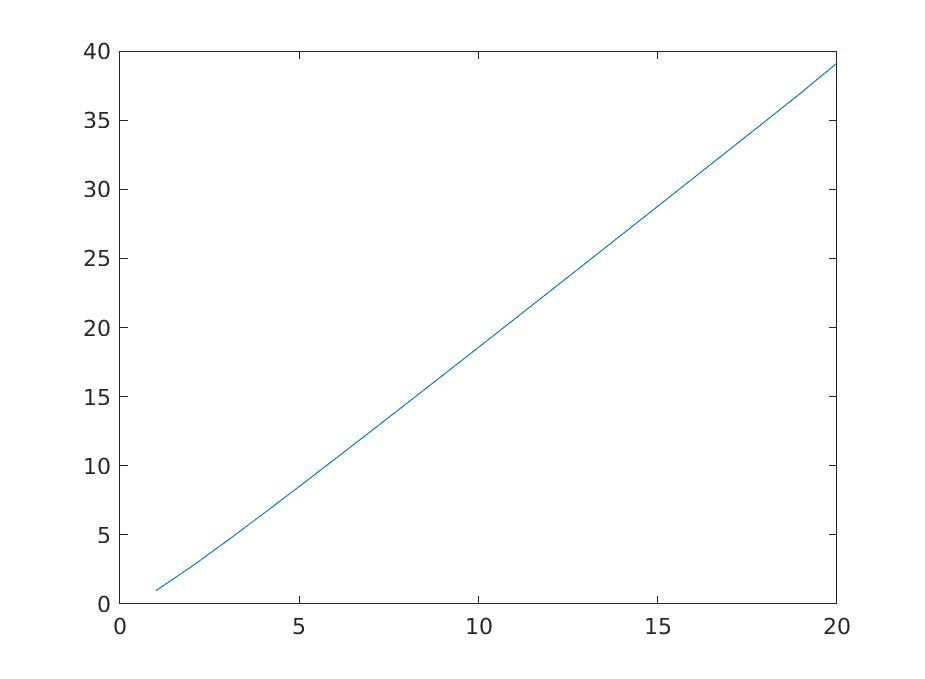
\includegraphics[scale=0.5]{Sup3_1_Plot.jpg}
b.)\newline
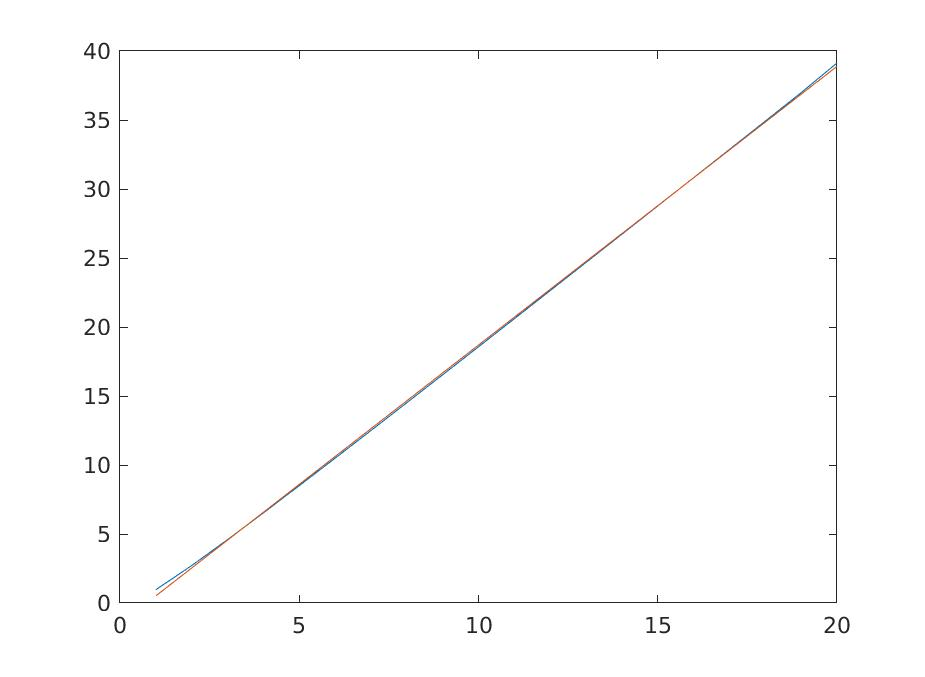
\includegraphics[scale=0.5]{Sup3_2.jpg}
Code:
\begin{lstlisting} [language = Matlab]
% Make the .../n vector
function x = HW9sup3(n)
    x = zeros(n+1, 1);
    for i = 0:n
        x(i+1) = i/n;
    end
end
% Make a vector of the condition numbers
conditions = zeros(20, 1);
for n = 1:20
    conditions(n) = cond(vander(HW9sup3(n)));
end
x = [1:20];
P = polyfit(x, log(conditions), 1)
% P(1) = m, P(2) = b
P =

   2.019377877332083  -1.501448611841827

\end{lstlisting}
c.)\newline
$C = e^{P(2)} = exp(P(2)) = 0.222807165159836$ and $a = e^{P(1)} = exp(P(1)) = 7.533636629343970$
\end{document}
